%!TEX root = ../Chapter2.tex
\section{Numerical Illustrations}\label{sec:t3c.experiments}
This section is aimed at illustrating our theoretical results and supporting the practical use of Bayesian sampling rules for fixed-confidence BAI.   %We also compare the different sampling rules.
%The main contribution of this paper is theoretical, thus the following experimental results are not for the purpose of showing the superiority of \TCC over existing methods, but rather supports a discussion on sampling rules.

We experiment with three different Bayesian sampling rules: \TCC, \TTTS and \TTEI, and we also include the Direct Tracking (\DT) rule of~\cite{garivier2016tracknstop} (which is adaptive to $\beta$), the \UGapE~\citep{gabillon2012ugape} algorithm, and a uniform baseline. In order to make a fair comparison, we use the Chernoff stopping rule~(\ref{eq:chernoffstoppingtime}) and associated recommendation rule for all of the sampling rules, including the uniform one, except for \UGapE which has its own stopping rule. Furthermore, we include a top-two variant of the Best Challenger (\BC) heuristic (see, e.g., \citealp{menard2019lma}). 

\BC selects the empirical best arm $\hat{I}_n$ with probability $\beta$ and the maximizer of $W_n(\hat{I}_n,j)$ with probability $1-\beta$, but also performs forced exploration (selecting any arm sampled less than $\sqrt{n}$ times at round $n$). \TCC can thus be viewed as a variant of \BC in which no forced exploration is needed to converge to $\bomega^\beta$, due to the noise added by replacing $\hat{I}_n$ with $I_n^{(1)}$.

We consider two simple instances with arms means given by $\bmu_1 = [0.5 \ 0.9 \ 0.4 \ 0.45 \ 0.44999]$, and $\bmu_2 = [1 \ 0.8 \ 0.75 \ 0.7]$ respectively. We run simulations for both Gaussian (with $\sigma=1$) and Bernoulli bandits with a risk parameter $\delta=0.01$. %In the Gaussian case, we set $\sigma=1$.
Figure~\ref{fig:confidence} reports the empirical distribution of $\tau_\delta$ under the different sampling rules, estimated over 1000 independent runs. 

\begin{figure*}[ht]
\centering
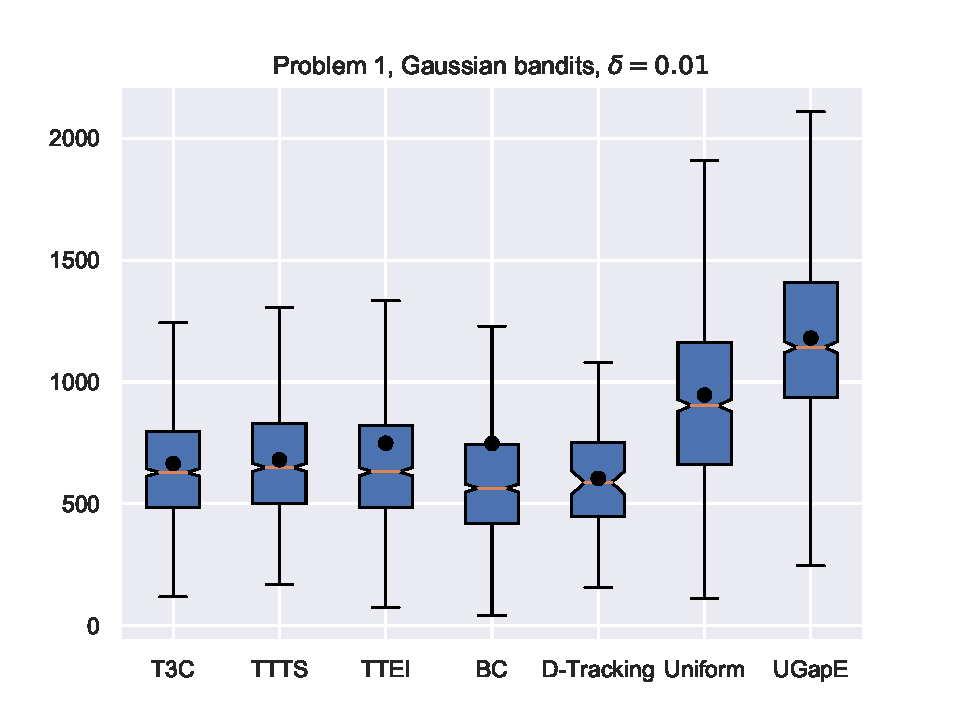
\includegraphics[clip, width= 0.49\textwidth]{Chapter3/img/gaussian1.pdf}
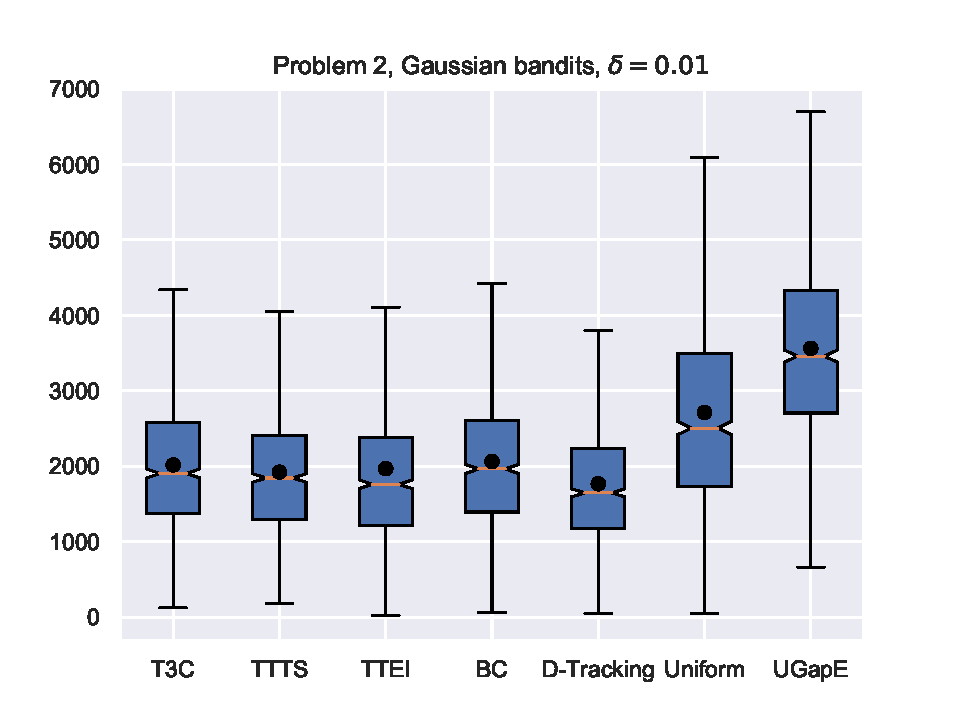
\includegraphics[clip, width= 0.49\textwidth]{Chapter3/img/gaussian2.pdf}
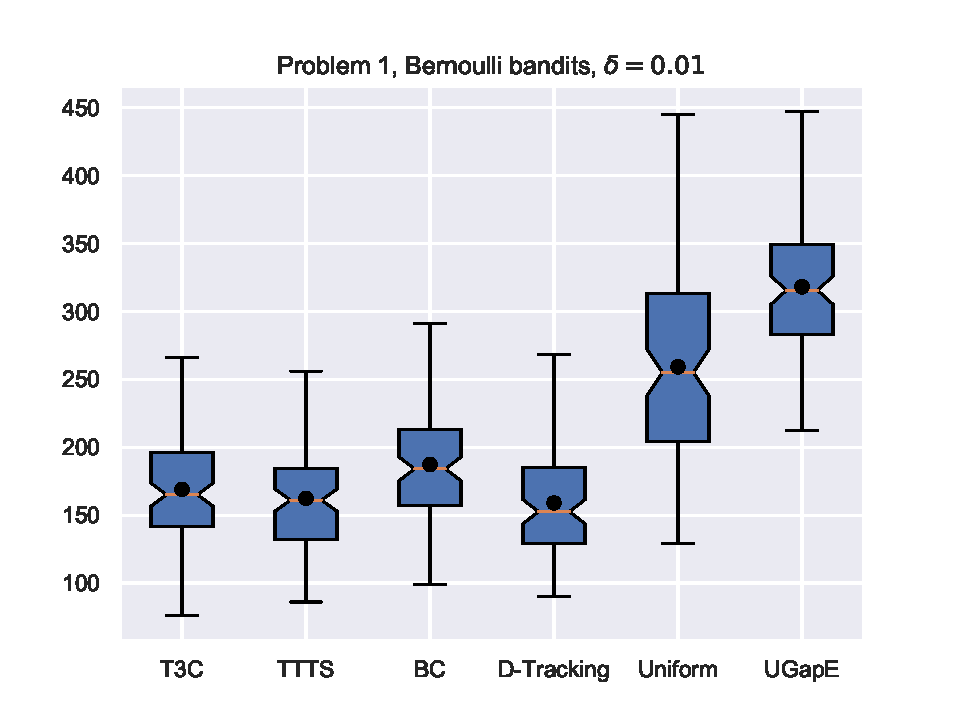
\includegraphics[clip, width= 0.49\textwidth]{Chapter3/img/bernoulli1.pdf}
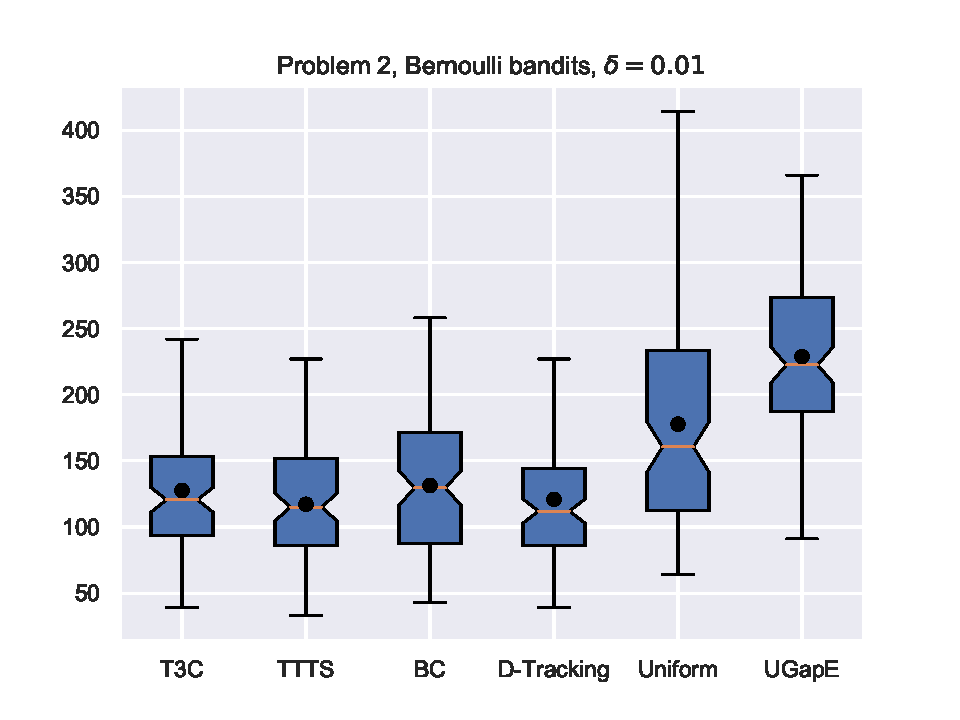
\includegraphics[clip, width= 0.49\textwidth]{Chapter3/img/bernoulli2.pdf}
\caption{Sample complexity of different BAI sampling rules over some random problem instances. Black dots represent means and oranges lines represent medians.}
\label{fig:confidence}
\end{figure*}

\begin{table*}[t!]
\centering
\small
%\def\arraystretch{1.2}
\begin{tabular}{|c|c|c|c|c|c|c|c|}
 \hline
 \textbf{Samp. rule} & \TCC & \TTTS & \TTEI & \BC & \texttt{D-T} & \texttt{Uniform} & \UGapE \\
 \hline
 \textbf{Exec. time (s)} & $1.6\times 10^{-5}$ & $2.3\times 10^{-4}$ & $1\times 10^{-5}$ & $1.4\times 10^{-5}$ & $1.3\times 10^{-3}$ & $6\times 10^{-6}$ & $5\times 10^{-6}$ \\
 \hline
\end{tabular}
\caption{Average execution time in seconds for different BAI sampling rules.}
\label{table:time}
\end{table*}

These figures provide several insights: (1) \TCC is competitive with, and sometimes slightly better than \TTTS and \TTEI in terms of sample complexity. (2) The \UGapE algorithm has a larger sample complexity than the uniform sampling rule, which highlights the importance of the stopping rule in the fixed-confidence setting. (3) The fact that \DT performs best is not surprising, since it converges to $\bomega^{\beta^\star}$ and achieves minimal sample complexity. However, in terms of computation time, \DT is much worse than other sampling rules, as can be seen in Table~\ref{table:time}, which reports the average execution time of one step of each sampling rule for $\mu_1$ in the Gaussian case. (4) \TTTS also suffers from computational costs, whose origins are explained in Section~\ref{sec:t3c.algorithm}, unlike \TCC and \TTEI. 
Although \TTEI is already computationally more attractive than \TTTS, its practical benefits are limited to the Gaussian case, since the \emph{Expected Improvement} (EI) does not have a closed form beyond this case and its approximation would be costly. In contrast, \TCC can be applied for other distributions.
